\section*{Comparison with priority queues}
\subsection*{The vEB tree as a priority queue}
The vEB tree can be used as a priority queue if we build some extra logic on top of it. Firstly a priority queue can contain several elements with the same priority, a search tree does not allow this. To get around this limitation we've build a new priority queue that can use any search tree as the underlying data structure. Ignoring intialization (this is just initializing the underlying search tree), we focus on the actual usage. Our priority queue support the following operations:

\begin{itemize}
  \item $void \textbf{ veb\_pq\_insert}(veb\_pq\_node * n, vebtree * tree)$
  \item $void \textbf{ veb\_pq\_delete}(vebtree * tree, veb\_pq\_node * node)$
  \item $veb\_pq\_node * \textbf{ veb\_pq\_deletemin}(vebtree * tree)$
  \item $void \textbf{ veb\_pq\_decrease\_key}(vebtree * tree, veb\_pq\_node * node, uint32\_t delta)$
\end{itemize}
A \textbf{veb\_pq\_data} is just a simple structure that contain a pointer to the first \textbf{veb\_pq\_node} in a linked list of nodes, and a counter, $n$ that is the number of nodes in the linked list. A \textbf{veb\_pq\_node} contains a pointer to the next and previous nodes, if any, and a pointer to the \textbf{veb\_pq\_data} holding the node; in particular, this last pointer allows us to check if a node is in the search tree or not, by seeing if the pointer is $NULL$. It also have an unsigned integer field that is the priority. Any auxilary data should also be included in this node - we just have a node number to indicate which node in the graph for our dijkstras algorithm it represent.

\begin{pseudocode}[Ovalbox]{veb\_pq\_insert}{node, tree}
data \GETS \text{succesor}(node.prio, tree)\\
\IF data.prio = node.prio
\THEN \text{insert $n$ into the linked list in $data$}
\ELSE 
\BEGIN
data \GETS \text{new veb\_pq\_data containing a single element, $node$} \\
  \text{insert}(data, tree)
\END
\end{pseudocode}

Let $T_{succ}(n)$ be the time for finding the successor to $n$, in the underlying datastructure, and let $T_{insert}(n)$ be the time to insert an element. Inserting $n$ into the linked list is a matter of updating a few, but constant number of pointers, so $O(1)$. The total time it takes to insert an element is $O(T_{succ}(n) + T_{insert}(n)$. With vEB trees as the underlying data structure, it's $O(\log \log U)$.

\begin{pseudocode}[Ovalbox]{veb\_pq\_delete}{node, tree}
\IF node.parent.n > 1
\THEN \text{then remove $node$ from the linked list}
\ELSE \text{remove}(node.parent, tree)
\end{pseudocode}

It is assumed we have a pointer to the node we want to delete. By the same argument as for \textbf{veb\_pq\_insert}, the time is $O(T_{remove}(n)$ which translates to $O(\log \log U)$.

\subsubsection*{\textbf{veb\_pq\_deletemin}}
Since vEB trees have a pointer to the minimum element, this can be fetched in constant time. The running time of \textbf{veb\_pq\_deletemin} is therefore $O(T_{remove}(n)) = O(\log \log U)$. The observant reader will notice that this means we can sort the integers $0, \dots, U$ in time $O(k \cdot \log \log U)$, where $k$ is the number of integers. So have we broken the $O(n \cdot \log n)$ barrier for comparison based integer sorting? No. In order to sort an arbitraty range of integers, we firstly need to build the vEB tree. Since this has size $O(U) = O(2^m)$, it takes $O(2^m)$ to build, where m is the bit length used for the vEB tree. This is clearly at least as large as $O(n)$. But for any fixed size integers set, we can sort efficiently by reusing the same vEB data structure.

\begin{pseudocode}[Ovalbox]{veb\_pq\_decreasekey}{node, delta, tree}
\text{veb\_pq\_delete}(node, tree)\\
node.prio \GETS n.prio - delta\\
\text{veb\_pq\_insert}(node, tree)
\end{pseudocode}

With a running time of $O(T_{delete}(n) + T_{insert}(n) = O(\log \log U)$.

All operations on our priority queue with vEB takes $O(\log \log U)$ time, except initialization.

\subsection*{Benchmarking}
From the previous project, we had a graph generating algorithm that would generate a large number of decrease calls, such that the binary heap would do $\log n$ work, i.e bubble the element, a leaf, all the way to the root. The Fibonacci heaps have the obvious advantage that they have amotized $O(1)$ time for secrease key calls, and vEB have $O(\log \log n)$. Question is, are the hidden constants too large for practical purposes?

For good messure we have also included a random graph, where each vertice has a 15\% chance of being connected to another vertice with the weight being between 1 and a chosen maximum.

We measured the running time using two different methods. One using normal absolute time measurement, the other one counting clock cycles. Curios to see which method had the lowest standard deviation we were surprised to discover that it increases using both methods quite rapidly as the graph sizes grow bigger.\newline

\subsubsection*{Dijkstra: Random graph VI SKAL TESTE OP TIL OG MED 100000 nodes her!!}
% GNUPLOT: LaTeX picture with Postscript
\begingroup
  \makeatletter
  \providecommand\color[2][]{%
    \GenericError{(gnuplot) \space\space\space\@spaces}{%
      Package color not loaded in conjunction with
      terminal option `colourtext'%
    }{See the gnuplot documentation for explanation.%
    }{Either use 'blacktext' in gnuplot or load the package
      color.sty in LaTeX.}%
    \renewcommand\color[2][]{}%
  }%
  \providecommand\includegraphics[2][]{%
    \GenericError{(gnuplot) \space\space\space\@spaces}{%
      Package graphicx or graphics not loaded%
    }{See the gnuplot documentation for explanation.%
    }{The gnuplot epslatex terminal needs graphicx.sty or graphics.sty.}%
    \renewcommand\includegraphics[2][]{}%
  }%
  \providecommand\rotatebox[2]{#2}%
  \@ifundefined{ifGPcolor}{%
    \newif\ifGPcolor
    \GPcolorfalse
  }{}%
  \@ifundefined{ifGPblacktext}{%
    \newif\ifGPblacktext
    \GPblacktexttrue
  }{}%
  % define a \g@addto@macro without @ in the name:
  \let\gplgaddtomacro\g@addto@macro
  % define empty templates for all commands taking text:
  \gdef\gplbacktext{}%
  \gdef\gplfronttext{}%
  \makeatother
  \ifGPblacktext
    % no textcolor at all
    \def\colorrgb#1{}%
    \def\colorgray#1{}%
  \else
    % gray or color?
    \ifGPcolor
      \def\colorrgb#1{\color[rgb]{#1}}%
      \def\colorgray#1{\color[gray]{#1}}%
      \expandafter\def\csname LTw\endcsname{\color{white}}%
      \expandafter\def\csname LTb\endcsname{\color{black}}%
      \expandafter\def\csname LTa\endcsname{\color{black}}%
      \expandafter\def\csname LT0\endcsname{\color[rgb]{1,0,0}}%
      \expandafter\def\csname LT1\endcsname{\color[rgb]{0,1,0}}%
      \expandafter\def\csname LT2\endcsname{\color[rgb]{0,0,1}}%
      \expandafter\def\csname LT3\endcsname{\color[rgb]{1,0,1}}%
      \expandafter\def\csname LT4\endcsname{\color[rgb]{0,1,1}}%
      \expandafter\def\csname LT5\endcsname{\color[rgb]{1,1,0}}%
      \expandafter\def\csname LT6\endcsname{\color[rgb]{0,0,0}}%
      \expandafter\def\csname LT7\endcsname{\color[rgb]{1,0.3,0}}%
      \expandafter\def\csname LT8\endcsname{\color[rgb]{0.5,0.5,0.5}}%
    \else
      % gray
      \def\colorrgb#1{\color{black}}%
      \def\colorgray#1{\color[gray]{#1}}%
      \expandafter\def\csname LTw\endcsname{\color{white}}%
      \expandafter\def\csname LTb\endcsname{\color{black}}%
      \expandafter\def\csname LTa\endcsname{\color{black}}%
      \expandafter\def\csname LT0\endcsname{\color{black}}%
      \expandafter\def\csname LT1\endcsname{\color{black}}%
      \expandafter\def\csname LT2\endcsname{\color{black}}%
      \expandafter\def\csname LT3\endcsname{\color{black}}%
      \expandafter\def\csname LT4\endcsname{\color{black}}%
      \expandafter\def\csname LT5\endcsname{\color{black}}%
      \expandafter\def\csname LT6\endcsname{\color{black}}%
      \expandafter\def\csname LT7\endcsname{\color{black}}%
      \expandafter\def\csname LT8\endcsname{\color{black}}%
    \fi
  \fi
  \setlength{\unitlength}{0.0500bp}%
  \begin{picture}(7200.00,5040.00)%
    \gplgaddtomacro\gplbacktext{%
      \csname LTb\endcsname%
      \put(946,1584){\makebox(0,0)[r]{\strut{} 0}}%
      \csname LTb\endcsname%
      \put(946,1983){\makebox(0,0)[r]{\strut{} 20}}%
      \csname LTb\endcsname%
      \put(946,2383){\makebox(0,0)[r]{\strut{} 40}}%
      \csname LTb\endcsname%
      \put(946,2782){\makebox(0,0)[r]{\strut{} 60}}%
      \csname LTb\endcsname%
      \put(946,3181){\makebox(0,0)[r]{\strut{} 80}}%
      \csname LTb\endcsname%
      \put(946,3580){\makebox(0,0)[r]{\strut{} 100}}%
      \csname LTb\endcsname%
      \put(946,3980){\makebox(0,0)[r]{\strut{} 120}}%
      \csname LTb\endcsname%
      \put(946,4379){\makebox(0,0)[r]{\strut{} 140}}%
      \csname LTb\endcsname%
      \put(1078,1364){\makebox(0,0){\strut{} 0}}%
      \csname LTb\endcsname%
      \put(1896,1364){\makebox(0,0){\strut{} 2000}}%
      \csname LTb\endcsname%
      \put(2714,1364){\makebox(0,0){\strut{} 4000}}%
      \csname LTb\endcsname%
      \put(3532,1364){\makebox(0,0){\strut{} 6000}}%
      \csname LTb\endcsname%
      \put(4349,1364){\makebox(0,0){\strut{} 8000}}%
      \csname LTb\endcsname%
      \put(5167,1364){\makebox(0,0){\strut{} 10000}}%
      \csname LTb\endcsname%
      \put(5985,1364){\makebox(0,0){\strut{} 12000}}%
      \csname LTb\endcsname%
      \put(6803,1364){\makebox(0,0){\strut{} 14000}}%
      \put(176,2981){\rotatebox{-270}{\makebox(0,0){\strut{}Time (ms)}}}%
      \put(3940,1034){\makebox(0,0){\strut{}Vertices}}%
      \put(3940,4709){\makebox(0,0){\strut{}Random graph standard deviation}}%
    }%
    \gplgaddtomacro\gplfronttext{%
      \csname LTb\endcsname%
      \put(5948,613){\makebox(0,0)[r]{\strut{}Binary}}%
      \csname LTb\endcsname%
      \put(5948,393){\makebox(0,0)[r]{\strut{}Fibonacci}}%
      \csname LTb\endcsname%
      \put(5948,173){\makebox(0,0)[r]{\strut{}van Emde Boas}}%
    }%
    \gplbacktext
    \put(0,0){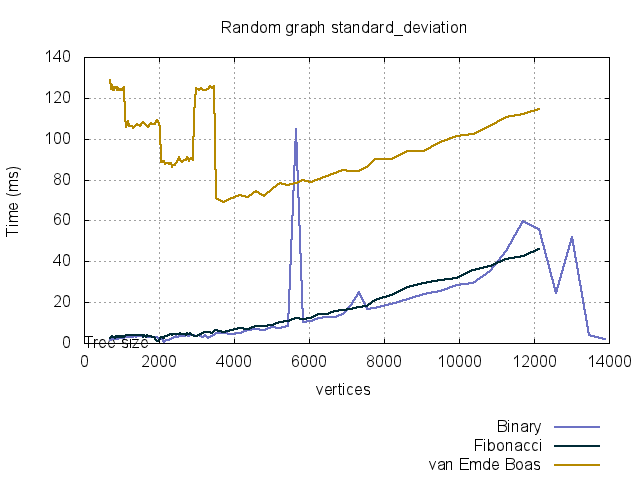
\includegraphics{graphs/random_standard_deviation_absolute}}%
    \gplfronttext
  \end{picture}%
\endgroup


The only exception being the random graph, when counting clock cycles.\newline
% GNUPLOT: LaTeX picture with Postscript
\begingroup
  \makeatletter
  \providecommand\color[2][]{%
    \GenericError{(gnuplot) \space\space\space\@spaces}{%
      Package color not loaded in conjunction with
      terminal option `colourtext'%
    }{See the gnuplot documentation for explanation.%
    }{Either use 'blacktext' in gnuplot or load the package
      color.sty in LaTeX.}%
    \renewcommand\color[2][]{}%
  }%
  \providecommand\includegraphics[2][]{%
    \GenericError{(gnuplot) \space\space\space\@spaces}{%
      Package graphicx or graphics not loaded%
    }{See the gnuplot documentation for explanation.%
    }{The gnuplot epslatex terminal needs graphicx.sty or graphics.sty.}%
    \renewcommand\includegraphics[2][]{}%
  }%
  \providecommand\rotatebox[2]{#2}%
  \@ifundefined{ifGPcolor}{%
    \newif\ifGPcolor
    \GPcolorfalse
  }{}%
  \@ifundefined{ifGPblacktext}{%
    \newif\ifGPblacktext
    \GPblacktexttrue
  }{}%
  % define a \g@addto@macro without @ in the name:
  \let\gplgaddtomacro\g@addto@macro
  % define empty templates for all commands taking text:
  \gdef\gplbacktext{}%
  \gdef\gplfronttext{}%
  \makeatother
  \ifGPblacktext
    % no textcolor at all
    \def\colorrgb#1{}%
    \def\colorgray#1{}%
  \else
    % gray or color?
    \ifGPcolor
      \def\colorrgb#1{\color[rgb]{#1}}%
      \def\colorgray#1{\color[gray]{#1}}%
      \expandafter\def\csname LTw\endcsname{\color{white}}%
      \expandafter\def\csname LTb\endcsname{\color{black}}%
      \expandafter\def\csname LTa\endcsname{\color{black}}%
      \expandafter\def\csname LT0\endcsname{\color[rgb]{1,0,0}}%
      \expandafter\def\csname LT1\endcsname{\color[rgb]{0,1,0}}%
      \expandafter\def\csname LT2\endcsname{\color[rgb]{0,0,1}}%
      \expandafter\def\csname LT3\endcsname{\color[rgb]{1,0,1}}%
      \expandafter\def\csname LT4\endcsname{\color[rgb]{0,1,1}}%
      \expandafter\def\csname LT5\endcsname{\color[rgb]{1,1,0}}%
      \expandafter\def\csname LT6\endcsname{\color[rgb]{0,0,0}}%
      \expandafter\def\csname LT7\endcsname{\color[rgb]{1,0.3,0}}%
      \expandafter\def\csname LT8\endcsname{\color[rgb]{0.5,0.5,0.5}}%
    \else
      % gray
      \def\colorrgb#1{\color{black}}%
      \def\colorgray#1{\color[gray]{#1}}%
      \expandafter\def\csname LTw\endcsname{\color{white}}%
      \expandafter\def\csname LTb\endcsname{\color{black}}%
      \expandafter\def\csname LTa\endcsname{\color{black}}%
      \expandafter\def\csname LT0\endcsname{\color{black}}%
      \expandafter\def\csname LT1\endcsname{\color{black}}%
      \expandafter\def\csname LT2\endcsname{\color{black}}%
      \expandafter\def\csname LT3\endcsname{\color{black}}%
      \expandafter\def\csname LT4\endcsname{\color{black}}%
      \expandafter\def\csname LT5\endcsname{\color{black}}%
      \expandafter\def\csname LT6\endcsname{\color{black}}%
      \expandafter\def\csname LT7\endcsname{\color{black}}%
      \expandafter\def\csname LT8\endcsname{\color{black}}%
    \fi
  \fi
  \setlength{\unitlength}{0.0500bp}%
  \begin{picture}(7200.00,5040.00)%
    \gplgaddtomacro\gplbacktext{%
      \csname LTb\endcsname%
      \put(1078,1584){\makebox(0,0)[r]{\strut{} 0}}%
      \csname LTb\endcsname%
      \put(1078,1864){\makebox(0,0)[r]{\strut{} 200}}%
      \csname LTb\endcsname%
      \put(1078,2143){\makebox(0,0)[r]{\strut{} 400}}%
      \csname LTb\endcsname%
      \put(1078,2423){\makebox(0,0)[r]{\strut{} 600}}%
      \csname LTb\endcsname%
      \put(1078,2702){\makebox(0,0)[r]{\strut{} 800}}%
      \csname LTb\endcsname%
      \put(1078,2982){\makebox(0,0)[r]{\strut{} 1000}}%
      \csname LTb\endcsname%
      \put(1078,3261){\makebox(0,0)[r]{\strut{} 1200}}%
      \csname LTb\endcsname%
      \put(1078,3541){\makebox(0,0)[r]{\strut{} 1400}}%
      \csname LTb\endcsname%
      \put(1078,3820){\makebox(0,0)[r]{\strut{} 1600}}%
      \csname LTb\endcsname%
      \put(1078,4100){\makebox(0,0)[r]{\strut{} 1800}}%
      \csname LTb\endcsname%
      \put(1078,4379){\makebox(0,0)[r]{\strut{} 2000}}%
      \csname LTb\endcsname%
      \put(1210,1364){\makebox(0,0){\strut{} 0}}%
      \csname LTb\endcsname%
      \put(2009,1364){\makebox(0,0){\strut{} 2000}}%
      \csname LTb\endcsname%
      \put(2808,1364){\makebox(0,0){\strut{} 4000}}%
      \csname LTb\endcsname%
      \put(3607,1364){\makebox(0,0){\strut{} 6000}}%
      \csname LTb\endcsname%
      \put(4406,1364){\makebox(0,0){\strut{} 8000}}%
      \csname LTb\endcsname%
      \put(5205,1364){\makebox(0,0){\strut{} 10000}}%
      \csname LTb\endcsname%
      \put(6004,1364){\makebox(0,0){\strut{} 12000}}%
      \csname LTb\endcsname%
      \put(6803,1364){\makebox(0,0){\strut{} 14000}}%
      \put(176,2981){\rotatebox{-270}{\makebox(0,0){\strut{}Time (ms)}}}%
      \put(4006,1034){\makebox(0,0){\strut{}Vertices}}%
      \put(4006,4709){\makebox(0,0){\strut{}Random graph standard_deviation}}%
    }%
    \gplgaddtomacro\gplfronttext{%
      \csname LTb\endcsname%
      \put(5948,613){\makebox(0,0)[r]{\strut{}Binary}}%
      \csname LTb\endcsname%
      \put(5948,393){\makebox(0,0)[r]{\strut{}Fibonacci}}%
      \csname LTb\endcsname%
      \put(5948,173){\makebox(0,0)[r]{\strut{}van Emde Boas}}%
    }%
    \gplbacktext
    \put(0,0){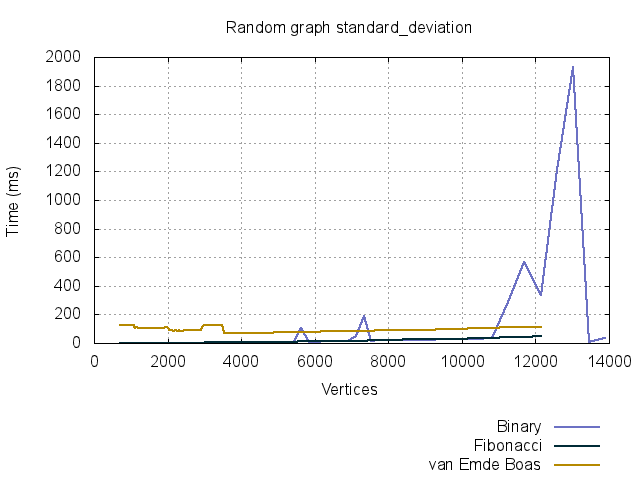
\includegraphics{graphs/random_standard_deviation_cycles}}%
    \gplfronttext
  \end{picture}%
\endgroup


We have yet to explain why this is happening. It is not a random deviation, our sample size is fairly large.\newline
% GNUPLOT: LaTeX picture with Postscript
\begingroup
  \makeatletter
  \providecommand\color[2][]{%
    \GenericError{(gnuplot) \space\space\space\@spaces}{%
      Package color not loaded in conjunction with
      terminal option `colourtext'%
    }{See the gnuplot documentation for explanation.%
    }{Either use 'blacktext' in gnuplot or load the package
      color.sty in LaTeX.}%
    \renewcommand\color[2][]{}%
  }%
  \providecommand\includegraphics[2][]{%
    \GenericError{(gnuplot) \space\space\space\@spaces}{%
      Package graphicx or graphics not loaded%
    }{See the gnuplot documentation for explanation.%
    }{The gnuplot epslatex terminal needs graphicx.sty or graphics.sty.}%
    \renewcommand\includegraphics[2][]{}%
  }%
  \providecommand\rotatebox[2]{#2}%
  \@ifundefined{ifGPcolor}{%
    \newif\ifGPcolor
    \GPcolorfalse
  }{}%
  \@ifundefined{ifGPblacktext}{%
    \newif\ifGPblacktext
    \GPblacktexttrue
  }{}%
  % define a \g@addto@macro without @ in the name:
  \let\gplgaddtomacro\g@addto@macro
  % define empty templates for all commands taking text:
  \gdef\gplbacktext{}%
  \gdef\gplfronttext{}%
  \makeatother
  \ifGPblacktext
    % no textcolor at all
    \def\colorrgb#1{}%
    \def\colorgray#1{}%
  \else
    % gray or color?
    \ifGPcolor
      \def\colorrgb#1{\color[rgb]{#1}}%
      \def\colorgray#1{\color[gray]{#1}}%
      \expandafter\def\csname LTw\endcsname{\color{white}}%
      \expandafter\def\csname LTb\endcsname{\color{black}}%
      \expandafter\def\csname LTa\endcsname{\color{black}}%
      \expandafter\def\csname LT0\endcsname{\color[rgb]{1,0,0}}%
      \expandafter\def\csname LT1\endcsname{\color[rgb]{0,1,0}}%
      \expandafter\def\csname LT2\endcsname{\color[rgb]{0,0,1}}%
      \expandafter\def\csname LT3\endcsname{\color[rgb]{1,0,1}}%
      \expandafter\def\csname LT4\endcsname{\color[rgb]{0,1,1}}%
      \expandafter\def\csname LT5\endcsname{\color[rgb]{1,1,0}}%
      \expandafter\def\csname LT6\endcsname{\color[rgb]{0,0,0}}%
      \expandafter\def\csname LT7\endcsname{\color[rgb]{1,0.3,0}}%
      \expandafter\def\csname LT8\endcsname{\color[rgb]{0.5,0.5,0.5}}%
    \else
      % gray
      \def\colorrgb#1{\color{black}}%
      \def\colorgray#1{\color[gray]{#1}}%
      \expandafter\def\csname LTw\endcsname{\color{white}}%
      \expandafter\def\csname LTb\endcsname{\color{black}}%
      \expandafter\def\csname LTa\endcsname{\color{black}}%
      \expandafter\def\csname LT0\endcsname{\color{black}}%
      \expandafter\def\csname LT1\endcsname{\color{black}}%
      \expandafter\def\csname LT2\endcsname{\color{black}}%
      \expandafter\def\csname LT3\endcsname{\color{black}}%
      \expandafter\def\csname LT4\endcsname{\color{black}}%
      \expandafter\def\csname LT5\endcsname{\color{black}}%
      \expandafter\def\csname LT6\endcsname{\color{black}}%
      \expandafter\def\csname LT7\endcsname{\color{black}}%
      \expandafter\def\csname LT8\endcsname{\color{black}}%
    \fi
  \fi
  \setlength{\unitlength}{0.0500bp}%
  \begin{picture}(7200.00,5040.00)%
    \gplgaddtomacro\gplbacktext{%
      \csname LTb\endcsname%
      \put(946,1584){\makebox(0,0)[r]{\strut{} 0}}%
      \csname LTb\endcsname%
      \put(946,2050){\makebox(0,0)[r]{\strut{} 20}}%
      \csname LTb\endcsname%
      \put(946,2516){\makebox(0,0)[r]{\strut{} 40}}%
      \csname LTb\endcsname%
      \put(946,2982){\makebox(0,0)[r]{\strut{} 60}}%
      \csname LTb\endcsname%
      \put(946,3447){\makebox(0,0)[r]{\strut{} 80}}%
      \csname LTb\endcsname%
      \put(946,3913){\makebox(0,0)[r]{\strut{} 100}}%
      \csname LTb\endcsname%
      \put(946,4379){\makebox(0,0)[r]{\strut{} 120}}%
      \csname LTb\endcsname%
      \put(1078,1364){\makebox(0,0){\strut{} 0}}%
      \csname LTb\endcsname%
      \put(1896,1364){\makebox(0,0){\strut{} 2000}}%
      \csname LTb\endcsname%
      \put(2714,1364){\makebox(0,0){\strut{} 4000}}%
      \csname LTb\endcsname%
      \put(3532,1364){\makebox(0,0){\strut{} 6000}}%
      \csname LTb\endcsname%
      \put(4349,1364){\makebox(0,0){\strut{} 8000}}%
      \csname LTb\endcsname%
      \put(5167,1364){\makebox(0,0){\strut{} 10000}}%
      \csname LTb\endcsname%
      \put(5985,1364){\makebox(0,0){\strut{} 12000}}%
      \csname LTb\endcsname%
      \put(6803,1364){\makebox(0,0){\strut{} 14000}}%
      \put(176,2981){\rotatebox{-270}{\makebox(0,0){\strut{}Time (ms)}}}%
      \put(3940,1034){\makebox(0,0){\strut{}Vertices}}%
      \put(3940,4709){\makebox(0,0){\strut{}Random graph samples}}%
    }%
    \gplgaddtomacro\gplfronttext{%
      \csname LTb\endcsname%
      \put(5948,613){\makebox(0,0)[r]{\strut{}Binary}}%
      \csname LTb\endcsname%
      \put(5948,393){\makebox(0,0)[r]{\strut{}Fibonacci}}%
      \csname LTb\endcsname%
      \put(5948,173){\makebox(0,0)[r]{\strut{}van Emde Boas}}%
    }%
    \gplbacktext
    \put(0,0){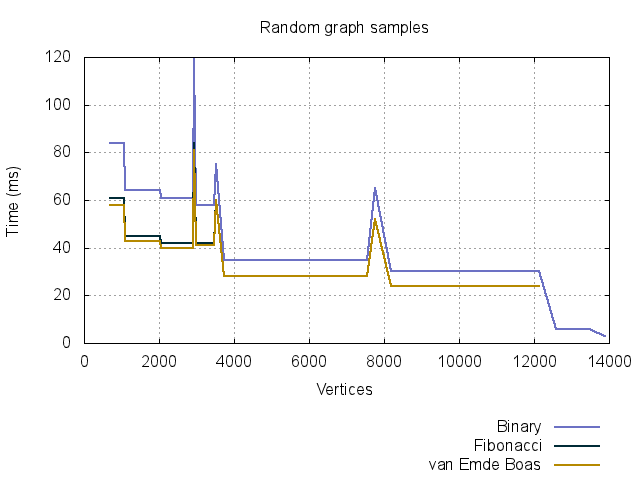
\includegraphics{graphs/random_samples_cycles}}%
    \gplfronttext
  \end{picture}%
\endgroup


As can be observed below, the graph does not bode well for van Emde Boas trees. It is slower by a constant of ~225 ms.\newline
% GNUPLOT: LaTeX picture with Postscript
\begingroup
  \makeatletter
  \providecommand\color[2][]{%
    \GenericError{(gnuplot) \space\space\space\@spaces}{%
      Package color not loaded in conjunction with
      terminal option `colourtext'%
    }{See the gnuplot documentation for explanation.%
    }{Either use 'blacktext' in gnuplot or load the package
      color.sty in LaTeX.}%
    \renewcommand\color[2][]{}%
  }%
  \providecommand\includegraphics[2][]{%
    \GenericError{(gnuplot) \space\space\space\@spaces}{%
      Package graphicx or graphics not loaded%
    }{See the gnuplot documentation for explanation.%
    }{The gnuplot epslatex terminal needs graphicx.sty or graphics.sty.}%
    \renewcommand\includegraphics[2][]{}%
  }%
  \providecommand\rotatebox[2]{#2}%
  \@ifundefined{ifGPcolor}{%
    \newif\ifGPcolor
    \GPcolorfalse
  }{}%
  \@ifundefined{ifGPblacktext}{%
    \newif\ifGPblacktext
    \GPblacktexttrue
  }{}%
  % define a \g@addto@macro without @ in the name:
  \let\gplgaddtomacro\g@addto@macro
  % define empty templates for all commands taking text:
  \gdef\gplbacktext{}%
  \gdef\gplfronttext{}%
  \makeatother
  \ifGPblacktext
    % no textcolor at all
    \def\colorrgb#1{}%
    \def\colorgray#1{}%
  \else
    % gray or color?
    \ifGPcolor
      \def\colorrgb#1{\color[rgb]{#1}}%
      \def\colorgray#1{\color[gray]{#1}}%
      \expandafter\def\csname LTw\endcsname{\color{white}}%
      \expandafter\def\csname LTb\endcsname{\color{black}}%
      \expandafter\def\csname LTa\endcsname{\color{black}}%
      \expandafter\def\csname LT0\endcsname{\color[rgb]{1,0,0}}%
      \expandafter\def\csname LT1\endcsname{\color[rgb]{0,1,0}}%
      \expandafter\def\csname LT2\endcsname{\color[rgb]{0,0,1}}%
      \expandafter\def\csname LT3\endcsname{\color[rgb]{1,0,1}}%
      \expandafter\def\csname LT4\endcsname{\color[rgb]{0,1,1}}%
      \expandafter\def\csname LT5\endcsname{\color[rgb]{1,1,0}}%
      \expandafter\def\csname LT6\endcsname{\color[rgb]{0,0,0}}%
      \expandafter\def\csname LT7\endcsname{\color[rgb]{1,0.3,0}}%
      \expandafter\def\csname LT8\endcsname{\color[rgb]{0.5,0.5,0.5}}%
    \else
      % gray
      \def\colorrgb#1{\color{black}}%
      \def\colorgray#1{\color[gray]{#1}}%
      \expandafter\def\csname LTw\endcsname{\color{white}}%
      \expandafter\def\csname LTb\endcsname{\color{black}}%
      \expandafter\def\csname LTa\endcsname{\color{black}}%
      \expandafter\def\csname LT0\endcsname{\color{black}}%
      \expandafter\def\csname LT1\endcsname{\color{black}}%
      \expandafter\def\csname LT2\endcsname{\color{black}}%
      \expandafter\def\csname LT3\endcsname{\color{black}}%
      \expandafter\def\csname LT4\endcsname{\color{black}}%
      \expandafter\def\csname LT5\endcsname{\color{black}}%
      \expandafter\def\csname LT6\endcsname{\color{black}}%
      \expandafter\def\csname LT7\endcsname{\color{black}}%
      \expandafter\def\csname LT8\endcsname{\color{black}}%
    \fi
  \fi
  \setlength{\unitlength}{0.0500bp}%
  \begin{picture}(7200.00,5040.00)%
    \gplgaddtomacro\gplbacktext{%
      \csname LTb\endcsname%
      \put(1078,1584){\makebox(0,0)[r]{\strut{} 0}}%
      \csname LTb\endcsname%
      \put(1078,2143){\makebox(0,0)[r]{\strut{} 500}}%
      \csname LTb\endcsname%
      \put(1078,2702){\makebox(0,0)[r]{\strut{} 1000}}%
      \csname LTb\endcsname%
      \put(1078,3261){\makebox(0,0)[r]{\strut{} 1500}}%
      \csname LTb\endcsname%
      \put(1078,3820){\makebox(0,0)[r]{\strut{} 2000}}%
      \csname LTb\endcsname%
      \put(1078,4379){\makebox(0,0)[r]{\strut{} 2500}}%
      \csname LTb\endcsname%
      \put(1210,1364){\makebox(0,0){\strut{} 0}}%
      \csname LTb\endcsname%
      \put(2009,1364){\makebox(0,0){\strut{} 2000}}%
      \csname LTb\endcsname%
      \put(2808,1364){\makebox(0,0){\strut{} 4000}}%
      \csname LTb\endcsname%
      \put(3607,1364){\makebox(0,0){\strut{} 6000}}%
      \csname LTb\endcsname%
      \put(4406,1364){\makebox(0,0){\strut{} 8000}}%
      \csname LTb\endcsname%
      \put(5205,1364){\makebox(0,0){\strut{} 10000}}%
      \csname LTb\endcsname%
      \put(6004,1364){\makebox(0,0){\strut{} 12000}}%
      \csname LTb\endcsname%
      \put(6803,1364){\makebox(0,0){\strut{} 14000}}%
      \put(176,2981){\rotatebox{-270}{\makebox(0,0){\strut{}Time (ms)}}}%
      \put(4006,1034){\makebox(0,0){\strut{}Vertices}}%
      \put(4006,4709){\makebox(0,0){\strut{}Random graph averages}}%
    }%
    \gplgaddtomacro\gplfronttext{%
      \csname LTb\endcsname%
      \put(5948,613){\makebox(0,0)[r]{\strut{}Binary}}%
      \csname LTb\endcsname%
      \put(5948,393){\makebox(0,0)[r]{\strut{}Fibonacci}}%
      \csname LTb\endcsname%
      \put(5948,173){\makebox(0,0)[r]{\strut{}van Emde Boas}}%
    }%
    \gplbacktext
    \put(0,0){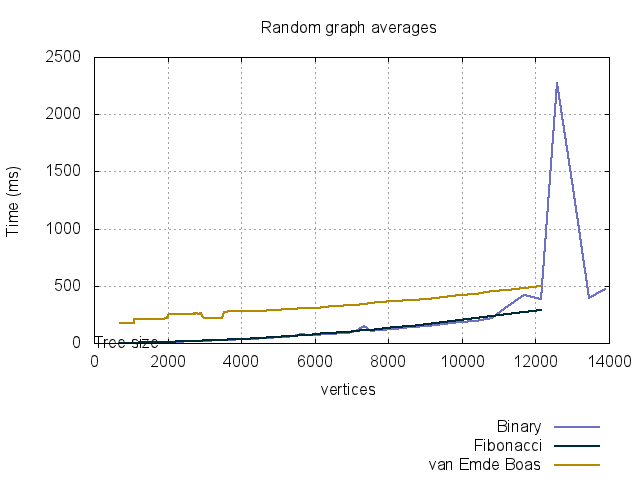
\includegraphics{graphs/random_averages_cycles}}%
    \gplfronttext
  \end{picture}%
\endgroup


\subsubsection*{Dijkstra: dkmax2 graph}
All this changes however, once we switch the graph generation algorithm to dkmax2. The algorithm we developed for previous assignment. As you can see, the van Emde Boas tree outperforms both the binary and fibonacci heap at approx. 6300 nodes. Curiously though, it have a rather, should we call it, funky, looking graph. It could be cache effects or something else. We have triple checked that it produce the correct output, so it's not a fatal bug that just make operations take constant time.\newline
% GNUPLOT: LaTeX picture with Postscript
\begingroup
  \makeatletter
  \providecommand\color[2][]{%
    \GenericError{(gnuplot) \space\space\space\@spaces}{%
      Package color not loaded in conjunction with
      terminal option `colourtext'%
    }{See the gnuplot documentation for explanation.%
    }{Either use 'blacktext' in gnuplot or load the package
      color.sty in LaTeX.}%
    \renewcommand\color[2][]{}%
  }%
  \providecommand\includegraphics[2][]{%
    \GenericError{(gnuplot) \space\space\space\@spaces}{%
      Package graphicx or graphics not loaded%
    }{See the gnuplot documentation for explanation.%
    }{The gnuplot epslatex terminal needs graphicx.sty or graphics.sty.}%
    \renewcommand\includegraphics[2][]{}%
  }%
  \providecommand\rotatebox[2]{#2}%
  \@ifundefined{ifGPcolor}{%
    \newif\ifGPcolor
    \GPcolorfalse
  }{}%
  \@ifundefined{ifGPblacktext}{%
    \newif\ifGPblacktext
    \GPblacktexttrue
  }{}%
  % define a \g@addto@macro without @ in the name:
  \let\gplgaddtomacro\g@addto@macro
  % define empty templates for all commands taking text:
  \gdef\gplbacktext{}%
  \gdef\gplfronttext{}%
  \makeatother
  \ifGPblacktext
    % no textcolor at all
    \def\colorrgb#1{}%
    \def\colorgray#1{}%
  \else
    % gray or color?
    \ifGPcolor
      \def\colorrgb#1{\color[rgb]{#1}}%
      \def\colorgray#1{\color[gray]{#1}}%
      \expandafter\def\csname LTw\endcsname{\color{white}}%
      \expandafter\def\csname LTb\endcsname{\color{black}}%
      \expandafter\def\csname LTa\endcsname{\color{black}}%
      \expandafter\def\csname LT0\endcsname{\color[rgb]{1,0,0}}%
      \expandafter\def\csname LT1\endcsname{\color[rgb]{0,1,0}}%
      \expandafter\def\csname LT2\endcsname{\color[rgb]{0,0,1}}%
      \expandafter\def\csname LT3\endcsname{\color[rgb]{1,0,1}}%
      \expandafter\def\csname LT4\endcsname{\color[rgb]{0,1,1}}%
      \expandafter\def\csname LT5\endcsname{\color[rgb]{1,1,0}}%
      \expandafter\def\csname LT6\endcsname{\color[rgb]{0,0,0}}%
      \expandafter\def\csname LT7\endcsname{\color[rgb]{1,0.3,0}}%
      \expandafter\def\csname LT8\endcsname{\color[rgb]{0.5,0.5,0.5}}%
    \else
      % gray
      \def\colorrgb#1{\color{black}}%
      \def\colorgray#1{\color[gray]{#1}}%
      \expandafter\def\csname LTw\endcsname{\color{white}}%
      \expandafter\def\csname LTb\endcsname{\color{black}}%
      \expandafter\def\csname LTa\endcsname{\color{black}}%
      \expandafter\def\csname LT0\endcsname{\color{black}}%
      \expandafter\def\csname LT1\endcsname{\color{black}}%
      \expandafter\def\csname LT2\endcsname{\color{black}}%
      \expandafter\def\csname LT3\endcsname{\color{black}}%
      \expandafter\def\csname LT4\endcsname{\color{black}}%
      \expandafter\def\csname LT5\endcsname{\color{black}}%
      \expandafter\def\csname LT6\endcsname{\color{black}}%
      \expandafter\def\csname LT7\endcsname{\color{black}}%
      \expandafter\def\csname LT8\endcsname{\color{black}}%
    \fi
  \fi
  \setlength{\unitlength}{0.0500bp}%
  \begin{picture}(7200.00,5040.00)%
    \gplgaddtomacro\gplbacktext{%
      \csname LTb\endcsname%
      \put(1078,1584){\makebox(0,0)[r]{\strut{} 0}}%
      \csname LTb\endcsname%
      \put(1078,1842){\makebox(0,0)[r]{\strut{} 500}}%
      \csname LTb\endcsname%
      \put(1078,2099){\makebox(0,0)[r]{\strut{} 1000}}%
      \csname LTb\endcsname%
      \put(1078,2357){\makebox(0,0)[r]{\strut{} 1500}}%
      \csname LTb\endcsname%
      \put(1078,2614){\makebox(0,0)[r]{\strut{} 2000}}%
      \csname LTb\endcsname%
      \put(1078,2872){\makebox(0,0)[r]{\strut{} 2500}}%
      \csname LTb\endcsname%
      \put(1078,3129){\makebox(0,0)[r]{\strut{} 3000}}%
      \csname LTb\endcsname%
      \put(1078,3387){\makebox(0,0)[r]{\strut{} 3500}}%
      \csname LTb\endcsname%
      \put(1078,3644){\makebox(0,0)[r]{\strut{} 4000}}%
      \csname LTb\endcsname%
      \put(1078,3902){\makebox(0,0)[r]{\strut{} 4500}}%
      \csname LTb\endcsname%
      \put(1078,4159){\makebox(0,0)[r]{\strut{} 5000}}%
      \csname LTb\endcsname%
      \put(1210,1364){\makebox(0,0){\strut{} 0}}%
      \csname LTb\endcsname%
      \put(2142,1364){\makebox(0,0){\strut{} 2000}}%
      \csname LTb\endcsname%
      \put(3074,1364){\makebox(0,0){\strut{} 4000}}%
      \csname LTb\endcsname%
      \put(4007,1364){\makebox(0,0){\strut{} 6000}}%
      \csname LTb\endcsname%
      \put(4939,1364){\makebox(0,0){\strut{} 8000}}%
      \csname LTb\endcsname%
      \put(5871,1364){\makebox(0,0){\strut{} 10000}}%
      \csname LTb\endcsname%
      \put(6803,1364){\makebox(0,0){\strut{} 12000}}%
      \put(176,2871){\rotatebox{-270}{\makebox(0,0){\strut{}Time (ms)}}}%
      \put(4006,1034){\makebox(0,0){\strut{}Vertices}}%
      \put(4006,4709){\makebox(0,0){\strut{}Decrease Key maximized v2 graph averages }}%
      \put(4006,4489){\makebox(0,0){\strut{}(Clock cycles)}}%
    }%
    \gplgaddtomacro\gplfronttext{%
      \csname LTb\endcsname%
      \put(5948,613){\makebox(0,0)[r]{\strut{}Binary}}%
      \csname LTb\endcsname%
      \put(5948,393){\makebox(0,0)[r]{\strut{}Fibonacci}}%
      \csname LTb\endcsname%
      \put(5948,173){\makebox(0,0)[r]{\strut{}van Emde Boas}}%
    }%
    \gplbacktext
    \put(0,0){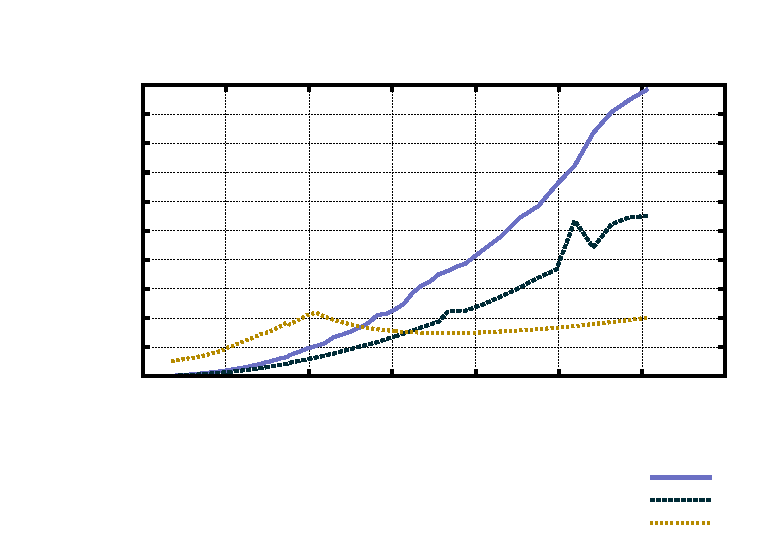
\includegraphics{graphs/dkmax2_averages_cycles}}%
    \gplfronttext
  \end{picture}%
\endgroup

